% created on 30/03/2020
% @author : ebazan
%\part{Color of the Textures}\label{part:local_color_of_texture}
%
%\section*{Introduction}
%We dedicate part \ref{part:global_color_texture} of this thesis to the study of the global distribution of color and texture information. In the case of color, we emphasize the importance of choosing a perceptual color space, while for texture, we show that Gabor filters satisfactorily characterize the properties of homogeneous textures. We show the aforementioned through two image retrieval systems that use color and texture information in conjunction with EMD to retrieve the most similar images. We also show that EMD is a metric that reflects the similarity between distributions in a perceptual way.
%
%However, the understanding of scenes (in a general way but particularly in the context of UAVs) is a more complex problem than the image retrieval systems presented in the previous part.
%First, the distribution of color and texture information in natural images is more complex. Since we are dealing with non-homogeneous images, an image may have objects with different colors and (or) textures. In addition, it is possible that one feature generates or is implicit in the other. For example, a repetitive variation between two colors seen very closely can be perceived as two objects, while seen at a longer distance, it can be perceived as the texture of a more complex object.
%
%In this final part of the thesis, we use the color and texture information again but in a different way. We explore the spectral decomposition of an image in a complex color space. With this strategy, we recover the local texture information of the objects in an image taking into account the luminance and chrominance information of the scene.
%
%This technique generates a space of balanced features that allows the recovery of the perceptual contours of the objects in an image and, consequently, segmentation. We show the versatility of this space using different techniques for object segmentation. While this framework is fully unsupervised, we show that it is also useful in identifying the importance of color and texture in human-made segmentations. Finally, we show that it is possible to obtain high-level features from this spectral decomposition.
%
%The main contributions of this part are:
%\begin{enumerate}
%	\item Extensive analysis of Gabor filters and their properties in the space-frequency domains.
%	\item Interactive tool for custom generation of 2D Gabor filters.
%	\item Generation of a feature space that includes the color and texture information of an image.
%	\item Unsupervised framework for natural image segmentation.
%	\item Tool for the interactive segmentation of images considering the information of color and texture.
%\end{enumerate}

\chapter{Spectral Image Decomposition}\label{ch:spectral_image_decomposition}

\section*{Résumé}
\noindent Ce chapitre utilise la théorie du signal et la transformée de Fourier pour générer une famille optimisée de filtres de Gabor. Le but est de récupérer autant d'informations que possible sur des textures d'une image dans le domaine fréquentiel sans affecter la localisation des informations. Nous présentons une analyse de la fonction de Gabor conforme au principe d'incertitude de Heisenberg. La méthodologie présentée dans ce chapitre générera des banques de filtres Gabor entièrement personnalisées.

\section*{Abstract}
\noindent This chapter uses signal theory and Fourier transform to generate an optimized family of Gabor filters. The goal is to retrieve as much information as possible about textures from an image in the frequency domain without affecting the information's location. We present an analysis of the Gabor function that complies with the Heisenberg uncertainty principle. The methodology presented in this chapter will generate fully customized Gabor filter banks. 

\section{Introduction}

The study and understanding of human vision have contributed to computer vision. Through neuropsychology, mathematical interpretations of the visual system have been developed, particularly the first area of the primary visual cortex, the so-called V1.

Novel experimental techniques \citep{DeAngelis.Ohzawa.ea:TN:1995} have made it possible to observe the activity of V1 and the modules involved in visual processes. It is known that the Receptive Field (RF) is in charge of formatting the optical signals for their interpretation. Physically, RF is the area of a visual neuron that responds to specific light stimuli. The RF response is known as the Receptive Profile (PR), and it can be positive and exciting or negative and exciting. Figure \ref{fig:V1_RP} shows the level curves of a neuron's receptor profile, showing positive responses in green and negative responses in red. 
Mathematically, the RP is a function $\varphi:  D \rightarrow \mathbb{R}$ defined in the RF domain $D$ that measures the neuron's response $\varphi(x,y)$ (as positive or negative) to the stimulations at the point $(x,y)$ \citep{Petitot:Neurogeometrie:2008}.
The transfer function of a neuron $\varphi(x,y)$ can be considered as a filter, e.g., the Gabor filter, that correctly replicates the behavior of the V1 receptive field (see Fig. \ref{fig:V1_RP_Gabor}).

\begin{figure}[!ht] 
	\centering
	\begin{subfigure}[b]{0.4\textwidth}
		\centering
		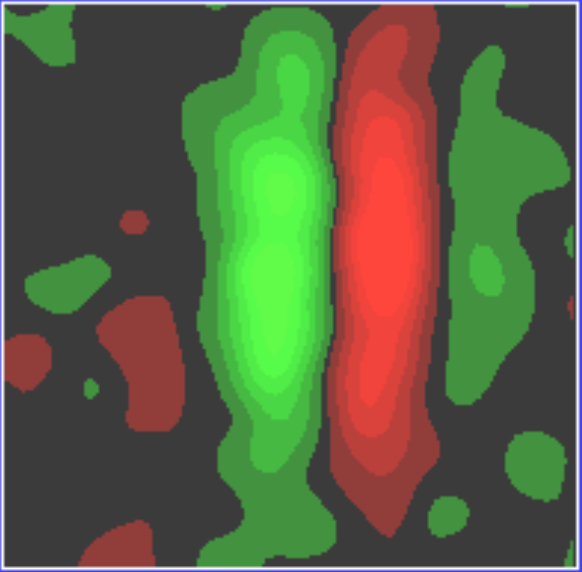
\includegraphics[width=\textwidth]{V1_RP2}
		\caption{Experimental level curves of RP}	
		\label{fig:V1_RP}
	\end{subfigure}
	\qquad %add desired spacing between images, e. g. ~, \quad, \qquad, \hfill etc. 
	%(or a blank line to force the subfigure onto a new line)
	\begin{subfigure}[b]{0.4\textwidth}
		\centering
		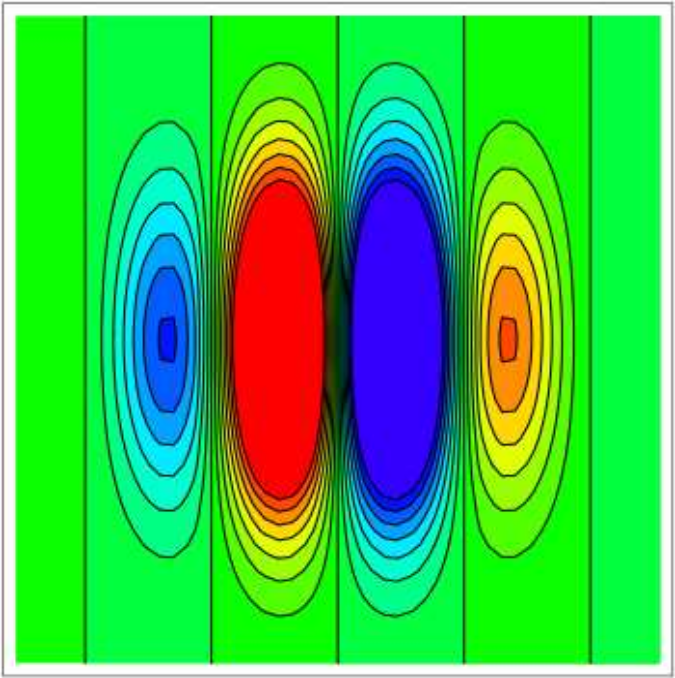
\includegraphics[width=\textwidth]{V1_RP_Gabor_model2}
		\caption{Gabor model of a RP }	
		\label{fig:V1_RP_Gabor}
	\end{subfigure}

  \caption{Receptive field of a simple visual neuron. Images from \citep{Petitot:Neurogeometrie:2008}.}
  \label{fig:simple_neuron_receptive_profil}
\end{figure}

In chapter \ref{ch:similarity_measures} we use the Gabor filter to extract global energy from homogeneous, i.e., stationary textures. This energy serves as the characteristic signature of the texture present in the image. In this chapter, motivated by its relationship with the human perception process, we delve into the study of Gabor filters. In particular, we are interested in its space-frequency properties to extract local texture features in natural images.

We carry out an analysis of the Gabor filters first from the point of view of signal theory to expose their properties and limits. Then, starting from the representation of the filters in 1-d, we propose a formulation of the filters that allow us to fully customize a family of 2-d filters depending on the application. The reformulation of Gabor filters allows dealing and take advantage of the aliasing and DC component. 
%(is this a conclusion?).

Using a Gabor filter family, we generate a feature bank that contains local information about the texture. As natural images contain color information, the proposed framework allows obtaining local texture features taking into account the luminance and the chrominance of an image. This strategy's novelty is that we consider color as a complex signal where we can measure the space-frequency distribution of a color texture. 

\section{The Gabor Filter as a Measurement Tool}\label{ch:gabor_filter_description}

This section presents a reminder of the signal theory applied to image processing for feature extraction. First, we show the reasons for restricting signal analysis in two predefined domains: time and frequency (for the 1-d case) and space and frequency (for the 2-d case). We especially recall Gabor filter theory and properties by showing how these filters are related to Heisenberg's uncertainty principle.

As we mentioned before, we use Gabor filters as a tool to measure the information that characterizes a signal. Since the signal carries relevant information at different points and scales (either in the spatial or space-frequency domain), a well-known strategy used in the literature is to create a filter bank that covers most of the spectrum to be able to reconstruct the original signal.

\subsection{Signals in Two Domains}
Bound by the Fourier transform, there are two equivalent representations of a signal (one-dimensional (1-d) or two-dimensional (2-d)). The first represents the signal as a function of time, while the second represents it as a function of frequency. These two representations carry the same information but in different ways; besides, we can go from one to another via the Fourier transform (or the inverse Fourier transform), making these special interest descriptions. We define the pair of 1-d Fourier transforms (FT) as follows
\begin{equation}\label{eq:fourier_transforms_1d}
    \begin{gathered}
        H(\upsilon) = \mathcal{F}\{h(t)\} = \int_{-\infty}^{\infty} h(t) e^{-j2\pi f t} dt \\
        h(t) = \mathcal{F}^{-1}\{H(\upsilon)\} = \int_{-\infty}^{\infty} H(\upsilon) e^{j2\pi f t} df 
    \end{gathered}
\end{equation}
while for the 2-d case, we define the FT as

\begin{equation}\label{eq:fourier_transforms_2d}
    \begin{gathered}
        H(u, v) = \mathcal{F}\{h(x, y)\} = \int_{-\infty}^{\infty} \int_{-\infty}^{\infty} h(x, y) e^{-j2\pi (ux + vy)} dx dy \\
        h(x, y) = \mathcal{F}^{-1}\{H(u, v)\} = \int_{-\infty}^{\infty} \int_{-\infty}^{\infty}  H(u, v) e^{j2\pi (ux + vy)} du dv 
    \end{gathered}
\end{equation}

%Both representations of the signal are somewhat ideal since the first operate at defined instants of time while the second operates on an infinite series of successive waves at defined frequencies \citep{Gabor:JIEE:1946}. 

It is evident that the function $h(t)$ (resp. $h(x, y)$) is located in both domains; however, it is also well known that no signal with compact support can have a finite Fourier transform and vice versa \citep{Bracewell:FourierBook:1999}, there is a particular uncertainty in the time and frequency locations of $h(t)$ (resp. space and frequency locations of $h(x, y)$). We developed and demonstrated the principle that defines this uncertainty (for signal processing and image processing) in the following section.%appendix \ref{ch:uncertainty_principle} of this document.

\subsection{The Uncertainty Principle in Image Processing}\label{ch:uncertainty_principle}

The uncertainty principle is one of the most famous ideas in quantum mechanics. An early incarnation of the uncertainty principle appeared in a 1927 paper by the German physicist Heisenberg. The uncertainty principle says that we cannot measure the position $(x)$ of a particle with absolute precision. The more accurately we know one of these values, the less accurately we know the other.

However, quantum mechanics' uncertainty principle is just a particular case of a more general compromise in simple everyday life phenomena involving waves. The central idea is connected with the interrelation between frequency and duration. For example, in the case of sound waves, if we want to identify the frequency of a musical note, the shorter the sound lasts in time, the less specific we can be about the exact frequency of the sound to find a more defined frequency, it would be necessary to listen to the sound for a longer time, in which case the locality measure loses its sense. In the language of signal processing, we can say that a short signal correlates highly with a wide range of frequencies, and only wide signals correlate with a short range of frequencies. Formally this is expressed as

\begin{equation}\label{eq:uncertainty_principle_rad}
	\Delta t\Delta \omega \geq \frac{1}{2}
\end{equation}

where $\Delta t$ is the duration of the signal in the time domain and $\Delta \omega$ is the bandwidth of the signal in the frequency domain \citep{Petrou.Sevilla:Book:2006}. The uncertainty principle then states: the spectral bandwidth product multiplied with the signal's time duration cannot be less than a particular minimum value. Considering the signal bandwidth in terms of frequency as $\Delta \upsilon$ where $\omega = 2\pi \upsilon$, the uncertainty principle is stated as 

\begin{equation}\label{eq:uncertainty_principle_freq}
	\Delta t\Delta \upsilon \geq \frac{1}{4\pi}
\end{equation}

The Heisenberg uncertainty principle can be mathematically proved in signal processing and image processing by \textbf{Parseval's identity}, where \textbf{Parseval's theorem}

\begin{equation}\label{eq:parseval_theorem}
	\int_{-\infty}^{\infty} h(t)^2 dt =  \frac{1}{2 \pi} \int_{-\infty}^{\infty} |H(\omega)|^2 d\omega =  \int_{-\infty}^{\infty} |H(\upsilon)|^2 d\upsilon
\end{equation}

where $h(t)$ is a function and $H(\upsilon)$ its the Fourier transform. 

The \textbf{energy content} of the signal described by $h(t)$ is defined as:

\begin{equation}\label{eq:energy_content_time}
    E_{\infty} \equiv \int_{-\infty}^{\infty}  h(t)^2 dt
\end{equation}


From the Parseval's identity this may be written as:

\begin{equation}\label{eq:energy_content_frequency}
    E_{\infty} =  \int_{-\infty}^{\infty} |H(\upsilon)|^2 d\upsilon
\end{equation}

By setting $\Delta t = t - t_0$, the \textbf{time dispersion} of the signal is given by

\begin{equation}\label{eq:time_dispersion_no_centered}
    (\Delta t)^2 \equiv \frac{1}{E_{\infty}} \int_{-\infty}^{\infty} (t-t_{0})^2 h(t)^2 dt
\end{equation}

where $t_0$ is the \textbf{center of gravity} of the signal defined by:

\begin{equation}\label{eq:center_of_gravity}
    t_0 \equiv \frac{1}{E_{\infty}} \int_{-\infty}^{\infty} t h(t)^2 dt
\end{equation}

and where if we shift the origin of $t$ so that $t_{0}=0$, then

\begin{equation}\label{eq:time_dispersion}
    (\Delta t)^2 = \frac{1}{E_{\infty}} \int_{-\infty}^{\infty} t^2 h(t)^2 dt
\end{equation}

In an analogous way for $\Delta \upsilon = \upsilon - f$, the \textbf{spectral bandwidth} of the signal is given by

\begin{equation}\label{eq:spectral_bandwidth_no_centered}
    (\Delta \upsilon)^2 \equiv \frac{1}{E_{\infty}} \int_{-\infty}^{\infty} (\upsilon-f)^2 |H(\upsilon)|^2 d\upsilon
\end{equation}

where $f$ is the \textbf{spectral center of gravity} of the signal defined by:

\begin{equation}\label{eq:spectral_center_of_gravity}
    f \equiv  \frac{2 \pi}{E_{\infty}} \int_{-\infty}^{\infty} f |H(\upsilon)|^2 d\upsilon
\end{equation}

if we consider $f=0$, the Eq. \eqref{eq:spectral_bandwidth_no_centered} becomes

\begin{equation}\label{eq:spectral_bandwidth}
    (\Delta \upsilon)^2 = \frac{1}{E_{\infty}} \int_{-\infty}^{\infty} f^2 |H(\upsilon)|^2 d\upsilon 
\end{equation}

If $h'(t)$ is the derivative of the function, its Fourier transform is $j2\pi f H(\upsilon)$. By applying the Parseval's identity (using the left and right terms in Eq. \eqref{eq:parseval_theorem})to the Fourier pair $h'(t)\longleftrightarrow j2\pi f H(\upsilon)$ we obtain:

\begin{equation}\label{eq:applyed_parseval_theorem}
    4 \pi^{2} \int_{-\infty}^{\infty} f^2 |H(\upsilon)|^2 d\upsilon =  \int_{-\infty}^{\infty} h'(t)^2 dt
\end{equation}

By substituting it in Eq. \eqref{eq:spectral_bandwidth}, we have:

\begin{equation}\label{eq:spectral_bandwidth2}
    (\Delta \upsilon)^2 = \frac{1}{4 \pi^{2} E_{\infty}} \int_{-\infty}^{\infty} h'(t)^2 dt
\end{equation}

We use Eqs. \eqref{eq:time_dispersion} and \eqref{eq:spectral_bandwidth2} to calculate:

\begin{equation}\label{eq:time_bandwidth_disp}
    (\Delta t)^2(\Delta \upsilon)^2 = \frac{1}{4 \pi^{2} E_{\infty}^{2}} \int_{-\infty}^{\infty} t^2h(t)^2 dt \int_{-\infty}^{\infty}h'(t)^2 dt
\end{equation}

Applying the Schwartz's inequality for the integrals on the right-hand side of Eq. \eqref{eq:time_bandwidth_disp}:

\begin{equation}\label{eq:schwartz_inequality}
    \int_{-\infty}^{\infty}t h(t)^2 dt \int_{-\infty}^{\infty}h'(t)^2 dt  \geq \biggr\rvert \int_{-\infty}^{\infty}t h(t)h'(t)^2 dt \biggr\rvert^{2}
\end{equation}

We may integrate by parts the integral on the right-hand side of Eq. \eqref{eq:schwartz_inequality}

\begin{equation}\label{eq:integr_by_parts}
    \int_{-\infty}^{\infty}t h(t) h'(t)^2 dt =  \frac{1}{2}t h(t)^2 \biggr\rvert_{-\infty}^{\infty} - \frac{1}{2} \int_{-\infty}^{\infty}h(t)^2 dt
\end{equation}

If $\lim_{t\rightarrow \infty} t h(t)^2=0$, the first term on the right-hand side of $\eqref{eq:integr_by_parts}$ vanishes and from equation $\eqref{eq:energy_content_time}$ we have

\begin{equation}\label{eq:energy_content_developped}
    \int_{-\infty}^{\infty} t h(t)h'(t) dt = -\frac{1}{2} E_{\infty}
\end{equation}

If we use this into $\eqref{eq:schwartz_inequality}$ and then into $\eqref{eq:time_bandwidth_disp}$ we obtain:

\begin{equation}\label{eq:uncertainty_principle_freq_square}
   (\Delta t)^2(\Delta \upsilon)^2 \geq \frac{1}{16\pi^{2}} 
\end{equation}

This is the mathematical statement of the uncertainty principle in signal processing \citep{Petrou.Sevilla:Book:2006}.

\subsection{1-d Gabor Filters}
The uncertainty principle shows that time and frequency are two fundamental domains and physically measurable quantities, but still idealizations if we consider one from the other's perspective. Frequency is a simple waveform in the time domain, but to be sharply defined in the frequency domain, it must be infinite in the time domain, i.e., a waveform that has always existed and will remain forever. In everyday life, it is complicated to find phenomena with these characteristics; it is more common to find signals that have properties from both domains; certainly, they have some frequency characteristics, but they also have a starting point, and after some time, these signals begin to fade away. This phenomenon motivated Dennis Gabor to represent signals simultaneously in time and frequency through the Gabor Elementary Function (GEF) \citep{Gabor:JIEE:1946}. The function represents the minimal quantum of information, i.e., the minimal amount of simultaneous information in time and frequency. In other words, it occupies the minimal area, given by a rectangle, in the time-frequency plane.  
%(see appendix \ref{ch:uncertainty_principle})

The Gabor function is derived form the uncertainty principle, therefore, it has a shape for which the product $\Delta t \Delta \upsilon$ assumes the smallest possible value. In other words, the Gabor function is the one that transforms inequality of Eq. \eqref{eq:uncertainty_principle_freq} into the equality $\Delta t \Delta \upsilon = \frac{1}{4 \pi}$. Then, the Gabor function is defined as the modulation product of a harmonic oscillation (a sinusoidal wave) of any frequency with a pulse of the form of a probability function (a Gaussian function) \citep{Gabor:JIEE:1946} and is represented as
\begin{equation}\label{eq:gabor_function_1d_time}
    g(t) =  e ^{-\alpha^2(t-t_0)^2} e ^{j 2 \pi f t + \phi}
\end{equation}
where $\alpha$ express the \textit{spread} and $t_0$ denotes the centroid of the Gaussian function, $f$ is the frequency of the sinusoidal wave, and $\phi$ defines the phase shift of the oscillation.

The Fourier transform of Eq. \eqref{eq:gabor_function_1d_time} defines the representation of the Gabor function in the frequency domain $G(\upsilon) = \mathcal{F}\{g(t)\}$ with the following analytical form

\begin{equation}\label{eq:gabor_function_1d_freq}
    G(\upsilon) =  \sqrt{\frac{\pi}{\alpha^2}} e ^{-\left(\frac{\pi}{\alpha}\right) ^{2} (\upsilon-f)^2} e ^{-j 2 \pi t_0 (\upsilon-f) + \phi}
\end{equation}

The equations \eqref{eq:gabor_function_1d_time} and \eqref{eq:gabor_function_1d_freq} show straightforward that the center of gravity $t_0$ is equal to \eqref{eq:center_of_gravity} and the spectral center of gravity $f$ is equal to \eqref{eq:spectral_center_of_gravity}, i.e., the Gabor functions follow Heisenberg's uncertainty principle.   

\begin{figure}[!ht] 

	\centering
	\begin{subfigure}[t]{\dimexpr0.9\textwidth+20pt\relax}
    	\makebox[20pt]{\raisebox{80pt} {\captext{(a)}} }%
    	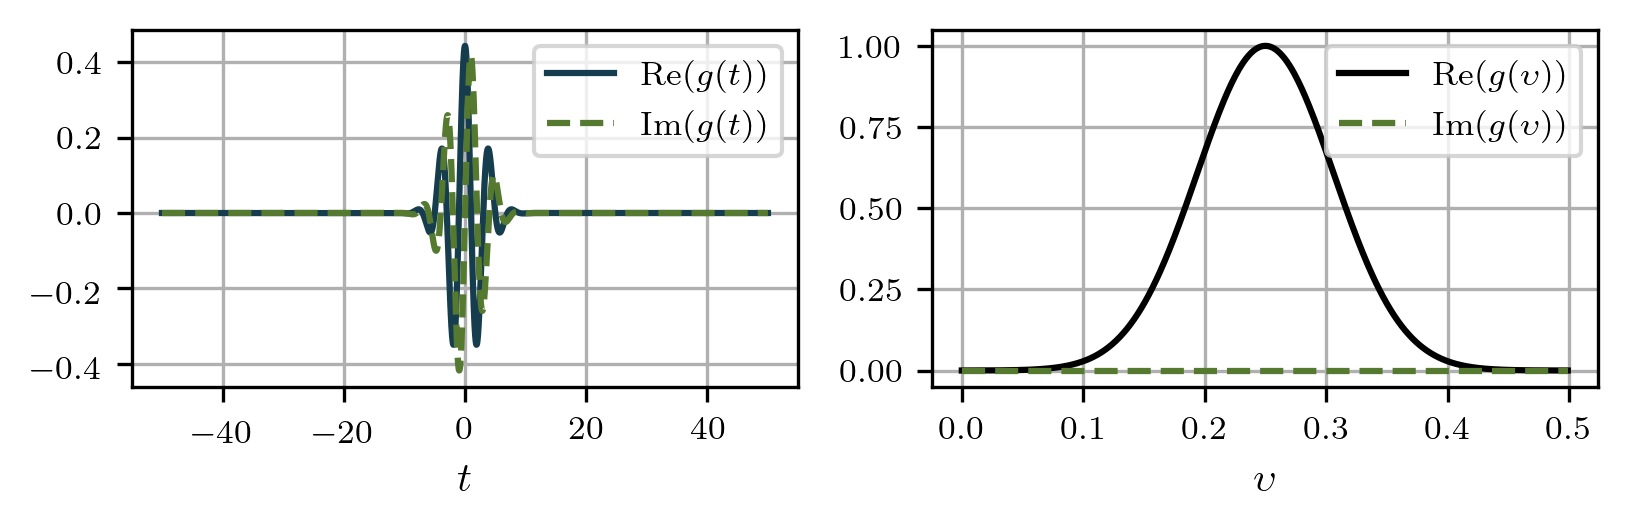
\includegraphics[width=\dimexpr\linewidth-20pt\relax]{1D_GaborFilter_hor_f4_g1}
    \end{subfigure}\vspace{-1em}
	\begin{subfigure}[t]{\dimexpr0.9\textwidth+20pt\relax}
    	\makebox[20pt]{\raisebox{80pt} {\captext{(b)}} }%
    	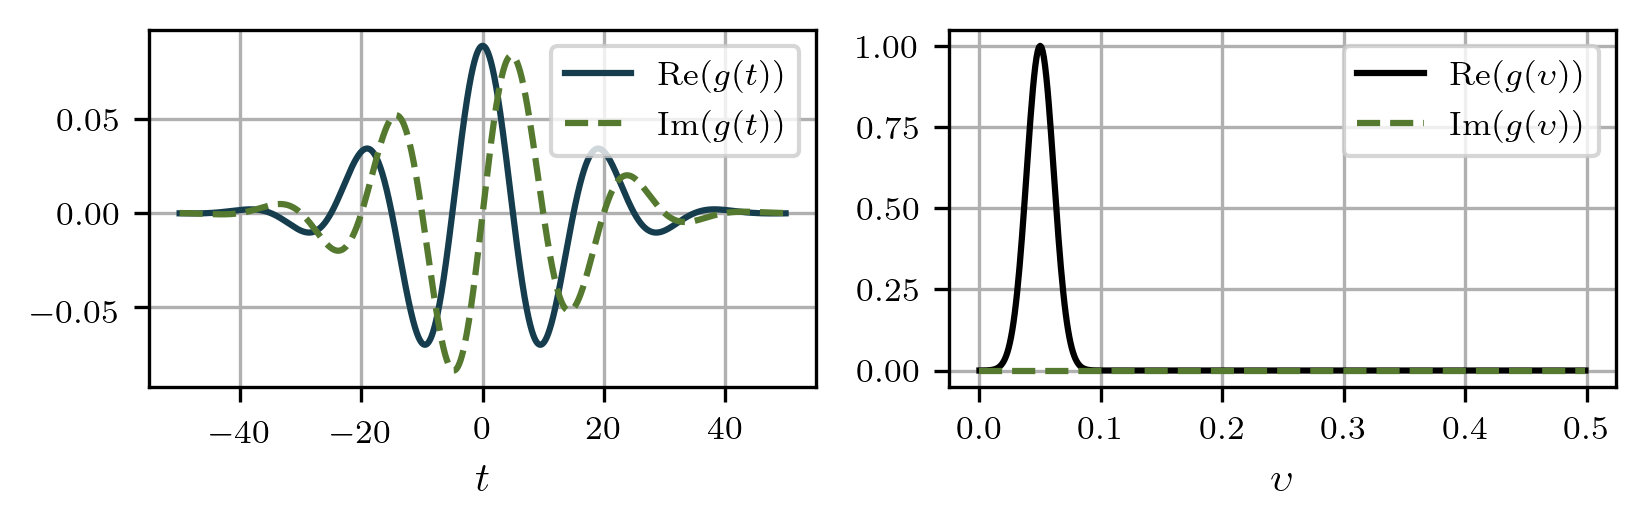
\includegraphics[width=\dimexpr\linewidth-20pt\relax]{1D_GaborFilter_hor_f20_g1}
    \end{subfigure}\vspace{-1em}
	\begin{subfigure}[t]{\dimexpr0.9\textwidth+20pt\relax}
    	\makebox[20pt]{\raisebox{80pt} {\captext{(c)}} }%
    	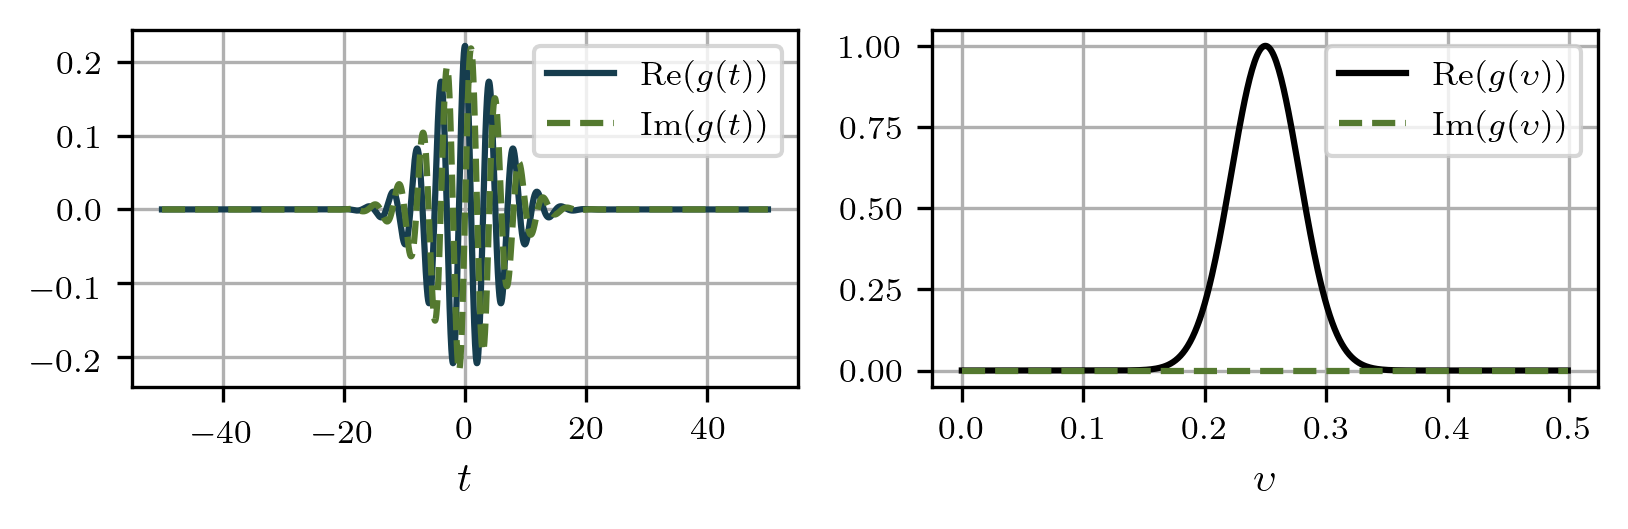
\includegraphics[width=\dimexpr\linewidth-20pt\relax]{1D_GaborFilter_hor_f4_g2}
    \end{subfigure}\vspace{-1em}
	\begin{subfigure}[t]{\dimexpr0.9\textwidth+20pt\relax}
    	\makebox[20pt]{\raisebox{80pt} {\captext{(d)}} }%
    	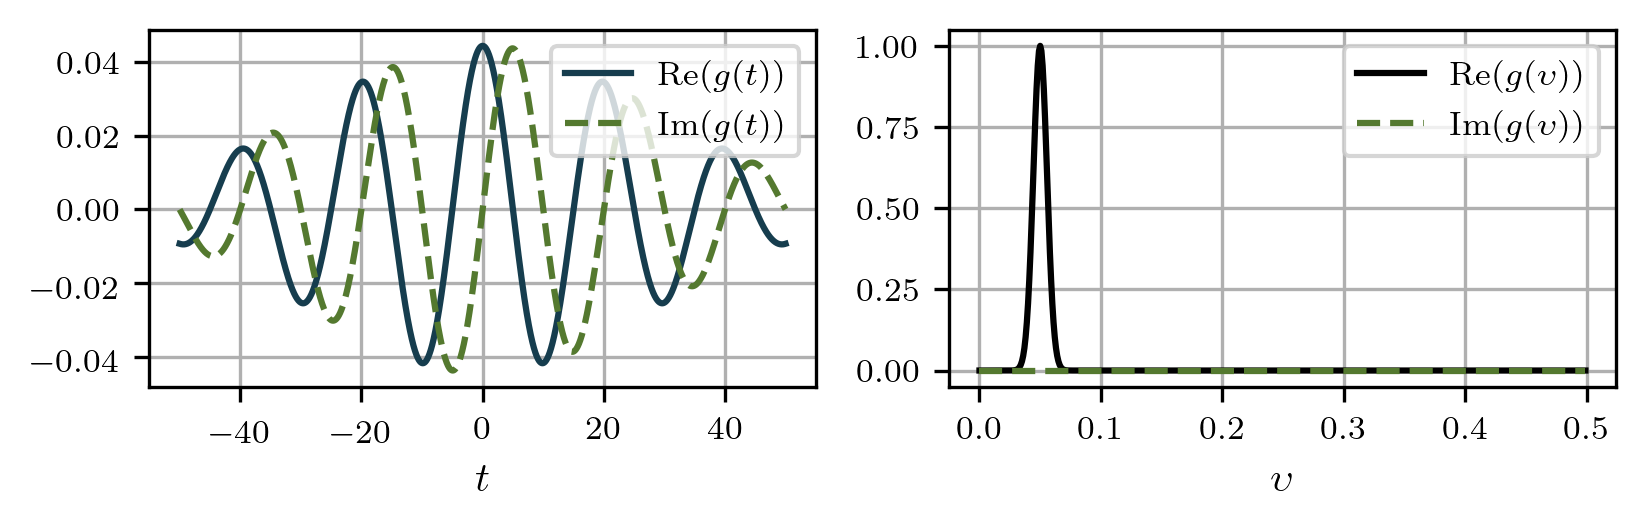
\includegraphics[width=\dimexpr\linewidth-20pt\relax]{1D_GaborFilter_hor_f20_g2}
    \end{subfigure}\vspace{-1em}
	
  	\caption{Visualization of the uncertainty principle in 1-d Gabor filters. First column: filters on the time domain, Second column: filters on the frequency domain. \captext{(a)} $f = 1/4$, $\gamma = 1$; \captext{(b)} $f = 1/20$, $\gamma = 1$; \captext{(c)} $f = 1/4$, $\gamma = 2$; \captext{(d)} $f = 1/20$, $\gamma = 2$.}
  \label{fig:examples_1D_GaborFilter}
\end{figure}

\subsubsection{Filter normalization} \label{subsec:filter_normalization}
We can define the Gabor filter more appropriately by taking the following justifications. First, we must remember that we use the Gabor function as a linear filter to analyze a signal. Under this condition, the temporal analysis of the signal is carried out using the convolution operator. Considering that the Gabor function is concentrated near the time instant $t_0$ and that a convolution centered at the origin is preferable, we consider $t_0 = 0$. Since there is no evidence that any specific phase would be more beneficial than any other, another parameter that we can omit is the phase shift $\phi$. Moreover, for the functions to be similar at all locations, the phase shift should depend on the location $t_0$, and thus, the phase shift can be removed from the origin-centered filter ($\phi$ = 0). Then, the Gabor filter function in its compact form is defined as 

\begin{equation}\label{eq:gabor_function_1d_timefreq_compact}
    \begin{gathered}
         g(t) =  e ^{-\alpha^2 t^2} e ^{j 2 \pi f t } \\
         G(\upsilon) =  \sqrt{\frac{\pi}{\alpha^2}} e ^{-\left(\frac{\pi}{\alpha}\right) ^{2} (\upsilon-f)^2} 
     \end{gathered}
\end{equation}

We can normalize the Gabor filter depending on the application we will use it. However, in this thesis, we use the general normalization based on the multi-domain representation property of the function following the subsequent conditions \citep{Boukerroui.Noble.ea:JMIV:2004}:

\begin{enumerate}
    \item Maximum condition:
        \begin{equation}\label{eq:maximun_condition}
            \max{|G(\upsilon)|} = 1
        \end{equation}
    \item Constant spectra condition:
        \begin{equation}\label{eq:constant_spectrum_condition}
            \int_{-\infty}^{\infty} |g(t)| dt = 1
        \end{equation}        
\end{enumerate}

From the equation \eqref{eq:gabor_function_1d_freq}, it is evident that the maximum response of the Gabor filter in the frequency domain is a function of $\sqrt{\pi/\alpha^2}$, therefore, its inverse
\begin{equation}\label{eq:normalization_factor}
    \sqrt{\frac{\alpha^2}{\pi}}
\end{equation}
can be used as the normalization factor in the time domain to fulfill the two conditions mentioned above. Then using the normalization factor \eqref{eq:normalization_factor}, the normalized Gabor filter is defined as

\begin{equation}\label{eq:gabor_function_1d_timefreq_normalized}
    \begin{gathered}
         g(t) =  \sqrt{\frac{\alpha^2}{\pi}} e ^{-\alpha^2 t^2} e ^{j 2 \pi f t } \\
         G(\upsilon) =  e ^{-\left(\frac{\pi}{\alpha}\right) ^2 (\upsilon-f)^2}
     \end{gathered}
\end{equation}

\begin{figure}[!ht]
	\centering
	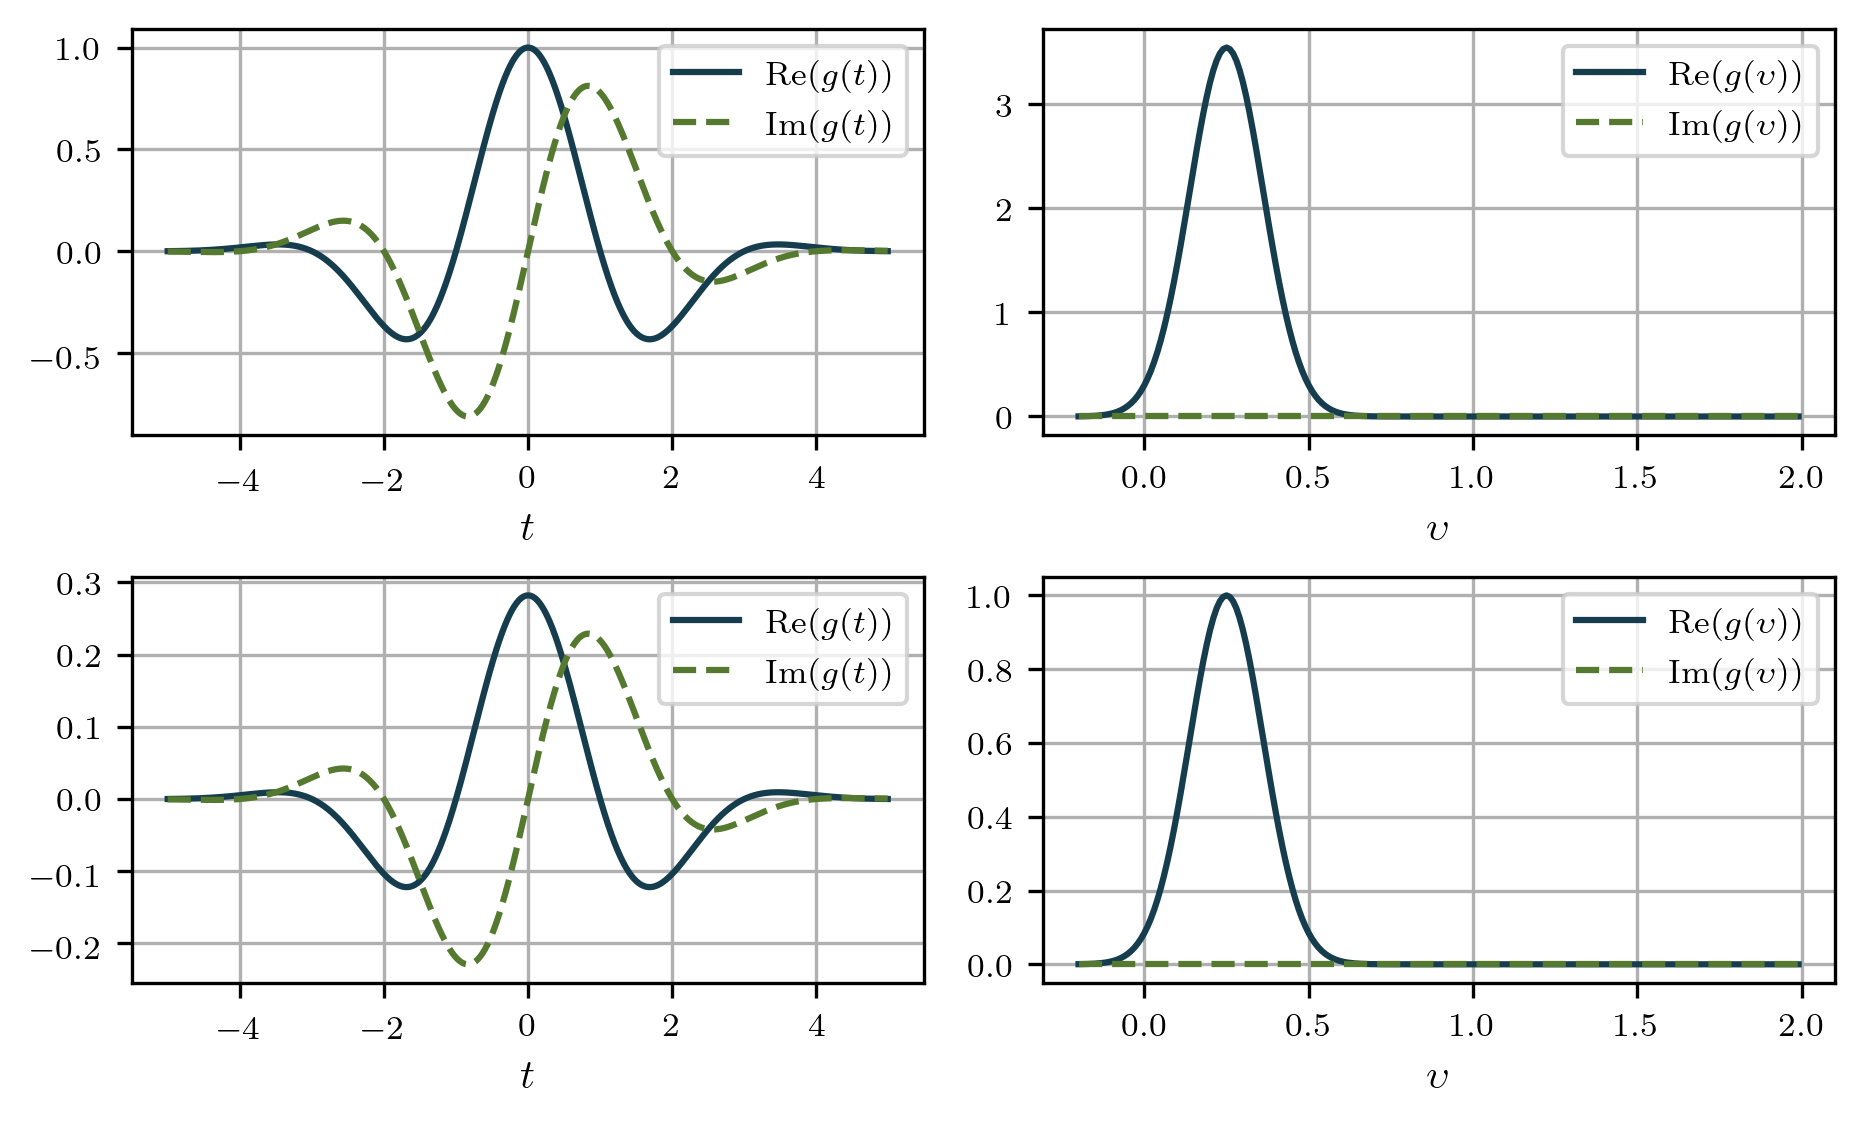
\includegraphics[width=0.9\textwidth]{GaborFilter_timefreq_1d_norm_efect}
	\caption{1-d Gabor filter in the time domain (first column) and in the frequency domain (second  column). From top to bottom: non-normalized and normalized Gabor filter with [$f =1/4$, $\alpha=0.5$, $t_0=0$].}\label{fig:GaborFilter_timefreq_norm_efect}
\end{figure}

Figure \ref{fig:GaborFilter_timefreq_norm_efect} shows a Gabor filter in the time and frequency domain before and after normalization following the two conditions described above. At this point, it is important to note that normalization is an essential step in the multi-spectral analysis and the feature extraction of a signal.

\subsubsection{Frequency filter spacing}\label{subsec:frequency_filter_spacing}
Our main interest in Gabor filters is the multi-spectral analysis of a function. We accomplish this by using multiple Gabor functions as filters that are tuned on several frequencies $f_m$. This group of filters is known as a \textit{Gabor filter bank}. The separation between the filter bank is defined through the half-response spatial frequency bandwidth $B_F$ measured between two central frequencies $f_1 < f_2$ \citep{Granlund:CGIP:1978}. This bandwidth is measured in octaves and we can express it as
\begin{equation}\label{eq:octave_spacing}
    B_f = \log_2 \left( \frac{f_2}{f_1} \right)
\end{equation}

The frequency bandwidth eq. \eqref{eq:octave_spacing} shows that the central frequencies $f_m$ must have a logarithmic relationship to maintain a homogeneous spacing between the filters. The scaling factor $k=2^{B_F}$ gives the logarithmic relationship, so the frequency of each filter ($f$) in this case corresponds to the scale information. Then we can write the central frequencies as
\begin{equation}
	f_m = k^{-m} f_{max}\textrm{,} \quad m = \{1, \cdots, M\} \label{eq:filterbank_frequencies}
\end{equation} 
where $f_m$ is the $m$th frequency, $f_{max}$ is the maximum desired frequency, $k>1$ is the frequency scaling factor, and $M$ is the total number of frequencies of the filter bank.

The octave spacing between two adjacent filters is an interesting property of the Gabor filters; however, the filters denoted by the Eqs. \eqref{eq:gabor_function_1d_timefreq_normalized} have a spread that only depends on the parameter $\alpha$, regardless of its central frequency $f$. This trait means that when implementing the Gabor function in a filter bank at different frequencies to obtain a multi-spectral decomposition of a signal, all of the filters will have the same spread in the frequency domain. We can see this effect in figure \ref{fig:filterbnk_octave_spacing}, where we show a filter bank with five central frequencies and an adjacent filter's spacing of one octave, that is, $M=5$ and $B_F = 1$. 


\subsubsection{Frequency crossing point}
The fact we choose the filter bank's central frequencies $f_m$ to have a constant separation causes two adjacent Gabor functions to intersect at a particular point on the frequency axis. For example, in a filter bank formed with two Gabor functions with central frequencies $f_1$ and $f_2$, the low cut-off frequency of the function at $f_1$ coincides with the high cut-off frequency of the function at $f_2$. Generally, in the literature, the crossing point $c_1$, corresponds to the points where the Gabor function has decreased half of its maximum value, i.e., $c_1= 1/2=0.5$ \citep{Granlund:CGIP:1978}. However, by setting the crossing point to half of the maximum value, the filter bank does not cover the input signal's entire spectrum. Consequently, the filter bank will not respond (or the response will be minimal) to artifacts oscillating between central frequencies.

We obtain the mathematical expression of this crossing point $c_1$ by defining a frequency interval $\Delta f$, representing the distance between points where the function $G(\upsilon)$ begins to decrease. The Gabor function has a peculiarity;  its analytical form in the frequency domain is completely defined by the Fourier transform of the normalized Gaussian function Eq. \eqref{eq:gabor_function_1d_timefreq_normalized}.

\begin{equation}\label{eq:1d_gaussian_function_freq}
    G(\upsilon) = w(\upsilon) = e ^{-\left(\frac{\pi}{\alpha}\right) ^{2} (\upsilon-f)^2}
\end{equation}
therefore, evaluating eq. \eqref{eq:1d_gaussian_function_freq} at $\upsilon = f + \frac{\Delta f}{2}$
\begin{equation}\label{eq:constant_crossing_point}
    G\left(f + \frac{\Delta f}{2}\right) = e^{-\left(\frac{\pi}{\alpha}\right)^2 \left(\frac{\Delta f}{2}\right)^2} = c_1 G(f) 
\end{equation}
we obtain the expression of the half-frequency interval 
\begin{equation}\label{eq:frequency_interval_crossing_point}
    \frac{\Delta f}{2} = \frac{\alpha}{\pi}\sqrt{\ln \left(\frac{1}{c_1}\right)}
\end{equation}
from which we obtain that the crossing point is defined as
\begin{equation}\label{eq:crossing_point}
    c_1 = e^{-\left(\frac{\alpha}{\pi} \right)^2 \left(\frac{\Delta f}{2}\right)^2 }
\end{equation}

This expression allows us to control the intersection point of two adjacent filters of the filter bank. Modifying the crossing point allows the generation of filter banks that cover (almost) the entire frequency spectrum, translating into a more faithful decomposition of the input signal.

\begin{figure}[!ht]
\centering
    \subcaptionbox{\label{fig:filterbnk_octave_spacing}}{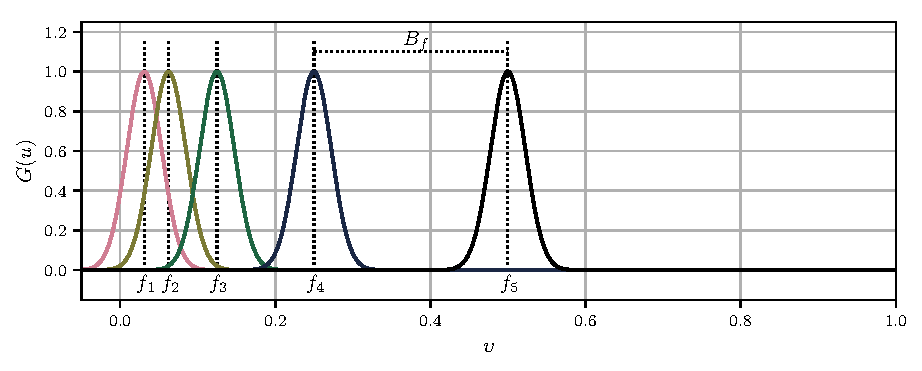
\includegraphics[width=\textwidth]{GaborFilterbank_freq_1d_octave_spacing.pdf}} \\
    \subcaptionbox{\label{fig:filterbnk_half_crossingpoint}}{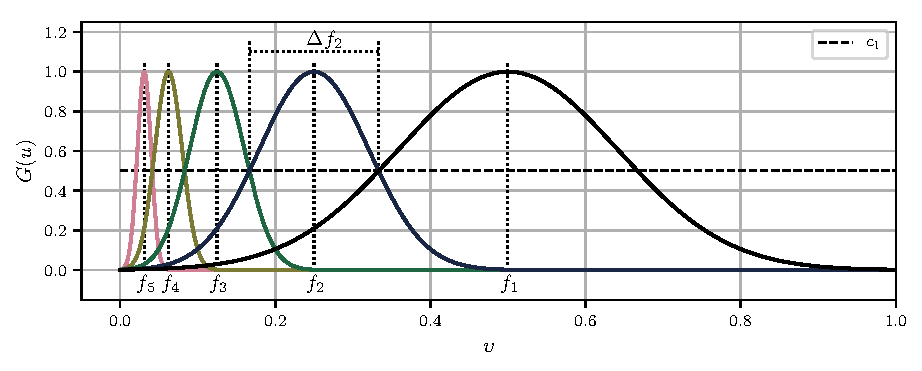
\includegraphics[width=\textwidth]{GaborFilterbank_freq_1d_half_crossingpoint.pdf}}\\
    \subcaptionbox{\label{fig:filterbnk_new_crossingpoint}}{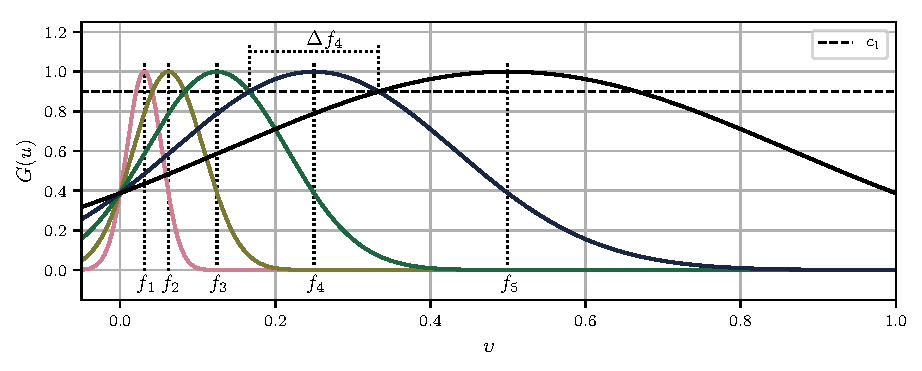
\includegraphics[width=\textwidth]{GaborFilterbank_freq_1d_new_crossingpoint.pdf}}
\caption{Filter spacing and crossing point effect represented on a bank of filters in the frequency domain: \captext{(a)} Separation of filters in octaves without crossing point between adjacent filters $[B_F=1, \alpha=0.1, c_1=-]$, \captext{(b)} High and low cut-off frequency points given by $\Delta f$ $[B_F=1, \alpha=f/\gamma, c_1=0.5]$, \captext{(c)} Filter bank behavior after changing the crossing point $[B_F=1, \alpha=f/\gamma, c_1=0.9]$.}\label{fig:1d_filterbank_spacing}
\end{figure}


\subsubsection{Effective and Adaptable Gaussian Envelope}
The full bandwidth $B_F$ (expressed in octaves) of a Gabor filter with center frequency $f$ and cut-off frequency interval $\Delta f$ is defined as \citep{Daugman:JOSA:1985}.
\begin{equation}\label{eq:frequency_bandwidth_interval}
    B_F = \log_2 \left( \frac{f + \frac{\Delta f}{2} }{f - \frac{\Delta f}{2}} \right)
\end{equation}

It is clear that using the half-frequency interval Eq. \eqref{eq:frequency_interval_crossing_point} into the frequency bandwidth Eq. \eqref{eq:frequency_bandwidth_interval}, we find an expression that introduces a relationship between the frequency bandwidth $B_F$, the central frequency $f$, and the spread of the Gabor filter $\alpha$.
\begin{equation}\label{eq:frequency_bandwidth}
    B_F = \log_2 \left( \frac{ \frac{f}{\alpha} \pi + \sqrt{\ln \left(\frac{1}{c_1}\right)} }{ \frac{f}{\alpha} \pi - \sqrt{\ln \left(\frac{1}{c_1}\right)} } \right)
\end{equation}
The relationship is noticeable through the ratio 
\begin{equation}\label{eq:gamma_ratio}
    \gamma = \frac{f}{\alpha}
\end{equation}

The ratio given in Eq. \ref{eq:gamma_ratio} allows generating Gabor filters of variable size as a function of the center frequency. For this, we must remember that the window size of a Gabor function is denoted by the effective width of a Gaussian function, which in the time domain has a form of
\begin{equation}\label{eq:1d_gaussian_function_time}
    w(t)=e^{-\frac{(t-t_0)^2}{2\sigma^2}}
\end{equation}

The Gaussian window Eq. \ref{eq:1d_gaussian_function_time} is infinite in its extent, so it is characterized by its locality $t_0$ and standard deviation $\sigma$, implicit in the Gabor function parameter $\alpha$ as $\alpha^2 = 1 / 2 \sigma^2$. By setting the standard deviation dependent on the frequency ratio and the central frequency, we find that
\begin{equation}
	\sigma = \frac{\gamma}{\sqrt{2}f} \label{eq:1D_Gaussian_envelope_width}
\end{equation} 
makes the Gabor's window adaptive as a function of the frequency.

In addition to adapting the filter size, with Eq. \eqref{eq:1D_Gaussian_envelope_width}, we make the Gabor filter effective; that is, we make the filter envelope correspond to the time (resp. spatial) support where the function's values are significant. We use the empirical \textit{three-sigma} rule \cite{Pukelsheim:AMSTAT:1994}, a conventional heuristic that expresses that nearly $99.7\%$ of the Gaussian distribution's energy lies within three standard deviations of the mean. Therefore, we define the shortest interval of the function that includes most of the energy as 
\begin{equation}
	\kappa = \lbrace p ~|~ x \in [-3\sigma, 3\sigma] \rbrace \label{eq:1D_gabor_support}
\end{equation}

The fact that the bank filters have the same width at all frequencies is not a problem, nor is it a requirement to analyze a signal with the Gabor function. However, making the filter width dependent on its frequency implies a multi-resolution analysis since the filters behave like a scaled version of each other. The advantages of an effective adaptative envelope are related to the computation time and the loss of information when we filter a signal with a Gabor filterbank. Figure \ref{fig:1D_space_Gaborfilterbank} illustrates the advantages of using a filter bank with adaptive and effective support (Fig. \ref{fig:1D_space_Gaborfilterbank_env}) versus a conventional filter bank (Fig. \ref{fig:1D_space_Gaborfilterbank_wo_env}). More precisely, in the case of constant envelope width, for the example $\kappa = \lbrace p ~|~ x \in [-50, 50] \rbrace$ (see Fig. \ref{fig:1D_space_Gaborfilterbank_wo_env}), the computation time of the responses is the same for all filter frequencies. In contrast, with the adaptive envelope, the calculation time is reduced for high frequencies since the envelope width is smaller (compare images on the first column of Fig. \ref{fig:1D_space_Gaborfilterbank}). Moreover, there is a risk of losing information from the original signal if the chosen envelope is not large enough for low frequencies to fit in(compare images on the last column of fig. \ref{fig:1D_space_Gaborfilterbank}). Using the adaptative and effective envelope width, we recover as much energy as possible from the signal by optimizing the response's computation time for each frequency $f$ of the filter.

\begin{figure}[!ht] 
	\centering
	\begin{subfigure}[b]{0.45\textwidth}
		\centering
		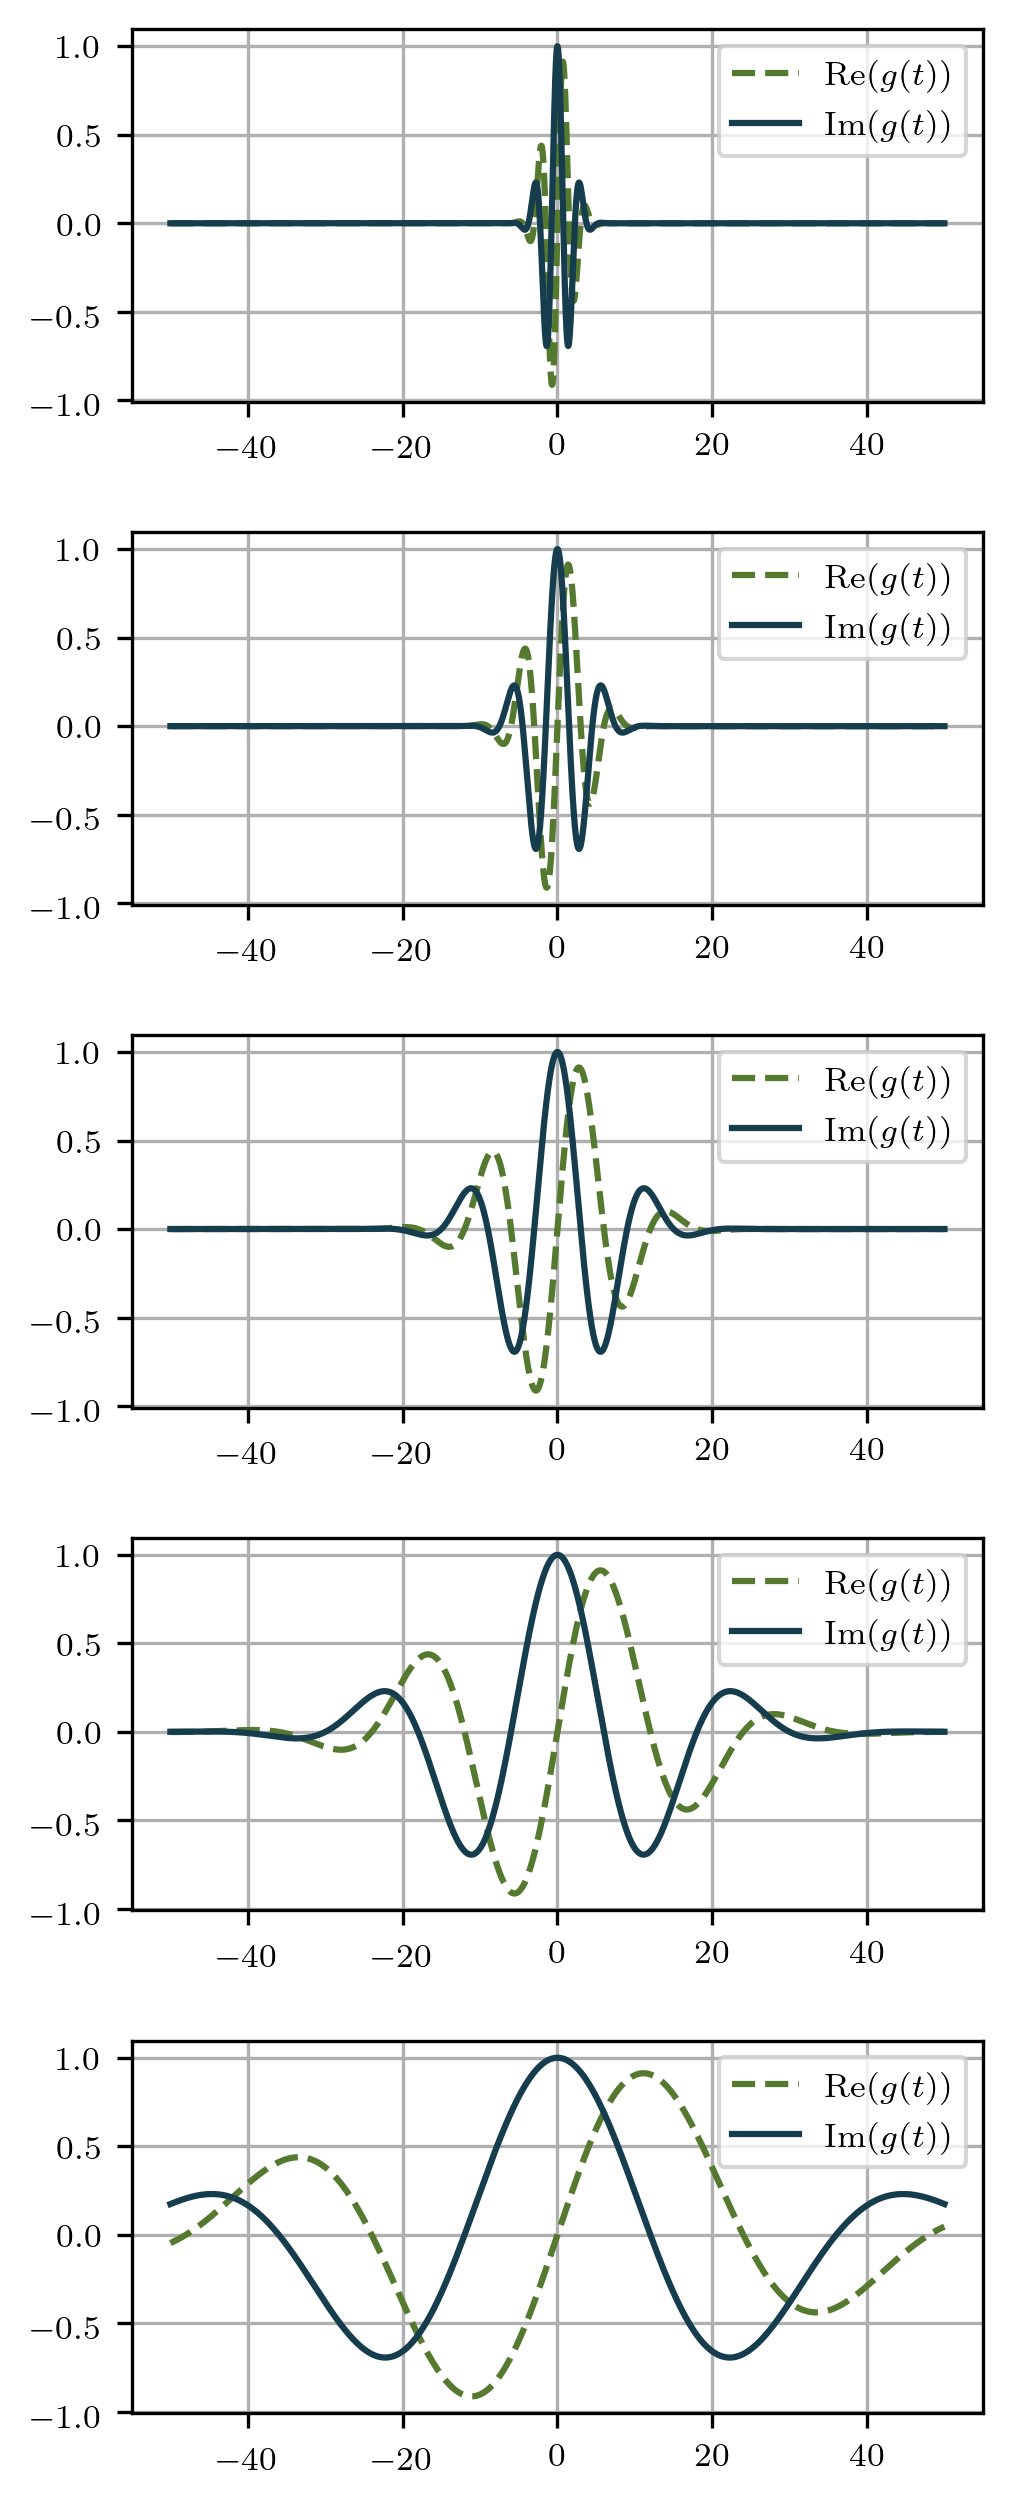
\includegraphics[width=\textwidth]{1D_space_GaborBank_m5_wo_env}
		\caption{$\kappa_{i} = \lbrace p: x \in [\pm 50] \rbrace$}
		\label{fig:1D_space_Gaborfilterbank_wo_env}
	\end{subfigure}
	\qquad %add desired spacing between images, e. g. ~, \quad, \qquad, \hfill etc. 
	%(or a blank line to force the subfigure onto a new line)
	\begin{subfigure}[b]{0.45\textwidth}
		\centering
		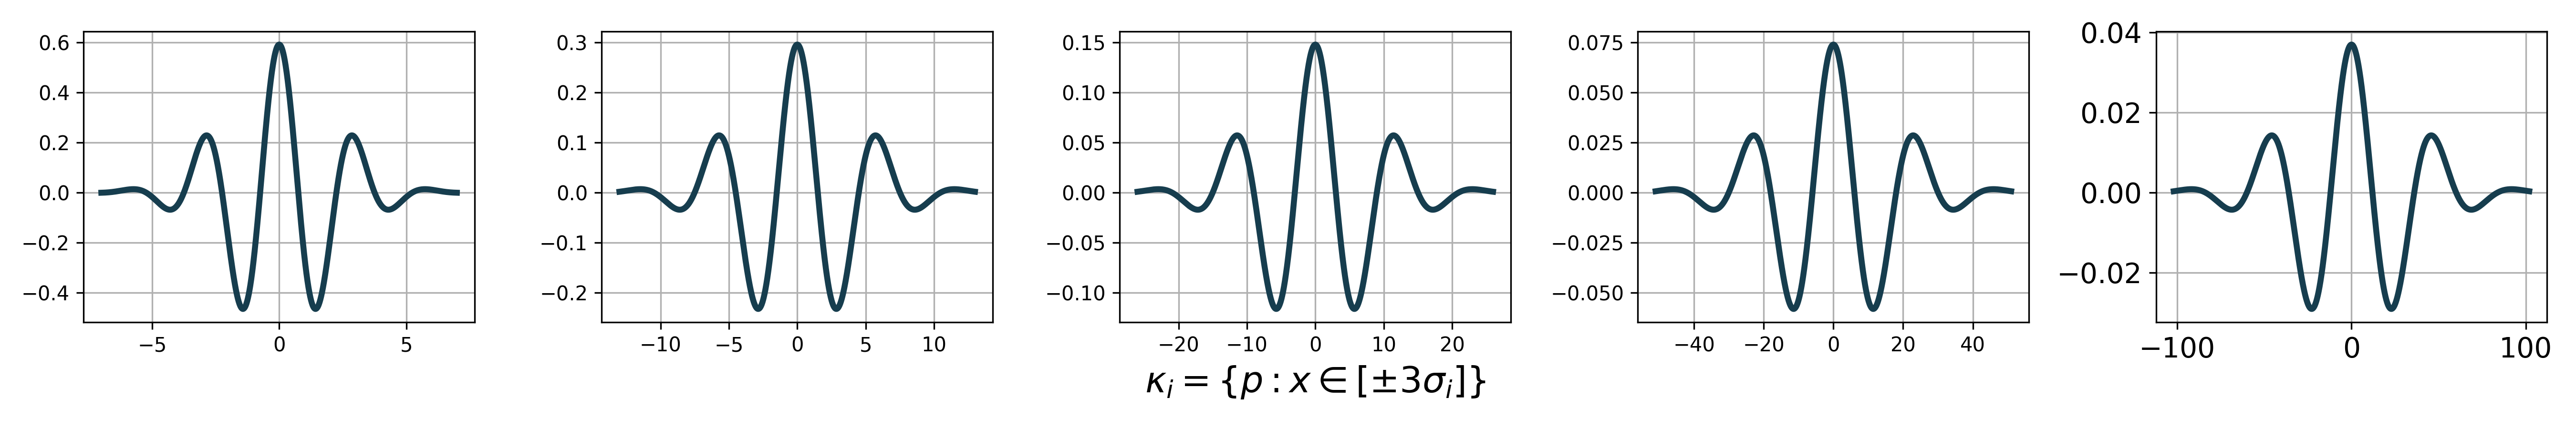
\includegraphics[width=\textwidth]{1D_space_GaborBank_m5_env}
		\caption{$\kappa_{i} = \lbrace p: x \in [\pm 3\sigma_{i}] \rbrace$}
		\label{fig:1D_space_Gaborfilterbank_env}
	\end{subfigure}

  \caption{Visual representation of the effective Gaussian envelope adaptation with filter bank with $M = 5$ frequencies in the space domain. \captext{(a)} Filter bank with no control over the envelope, \captext{(b)} Filter bank with control over the envelope's effective width.}
  \label{fig:1D_space_Gaborfilterbank}
\end{figure}


\subsubsection{Optimized 1-d Gabor function}
Gathering the different modifications of Gabor functions developed in the previous sections, we can define an optimized 1-d Gabor function as follows
\begin{equation}\label{eq:gabor_function_1d_timefreq_bank}
    \begin{gathered}
         g(t) =  \frac{f}{\gamma \sqrt{\pi}} e ^{-\left(\frac{f}{\gamma}\right)^2 t^2} e ^{j 2 \pi f t } \\
         G(\upsilon) =  e ^{-\left(\frac{\gamma \pi}{f}\right) ^2 (\upsilon-f)^2}
     \end{gathered}
\end{equation}

This Gabor function representation allows generating filter banks normalized by the maximum spectrum condition and homogeneously distributed in the frequency domain. Besides, a filter bank generated with the Gabor function Eq. \eqref{eq:gabor_function_1d_timefreq_bank} integrates the frequency crossing point allowing a quasi-total and almost flat coverage of the frequency spectrum, occupying the most relevant part of the filter using an adaptive window. A possible disadvantageous effect of this approach is the ripple between the filter bank's filters; however, we must remember that the filters proposed here are normalized concerning the size of the support (Gaussian window) and the central frequency of each filter. Therefore, even though a filter responds to different frequencies, textures close to the filter's center frequency are weighted. Additionally, the ripple effect occurs more frequently when decreasing the bandwidth of the filter bank. Moreover, this effect can be reduced by applying a halfwave rectification or, more generally called a thresholding \citep{Petkov:FGCS:1995}, \citep{Grigorescu.Petkov.ea:TIP:2003} \citep{Kruizinga.Petkov:TIP:1999}.

Figure \ref{fig:1d_filterbank_spacing} shows three examples of filter banks in the frequency domain.  Particulary, figure \ref{fig:filterbnk_octave_spacing} shows a bank without the relationship between the effective width and the central frequency of the filter, whereas the figures \ref{fig:filterbnk_half_crossingpoint} and \ref{fig:filterbnk_new_crossingpoint} show the interdependence between $\alpha$, $B_F$, $f$ and $c_1$ and the behavior of the bank with a different crossing point.

\subsection{2-d Gabor Filters}
The generalization of the Gabor function's theory from 1-d to 2-d is straightforward. First, we replace the time variable $t$ with the pair of spatial coordinates $(x, y)$ and the frequency variable $f$ with the pair of frequency variables $(u, v)$. Then, as for the 1-d case, the 2-d Gabor functions follows the Heisenberg principle where the uncertainty measures for the spatial and spatial-frequency domains are expressed in terms of $\Delta x$, $\Delta y$, $\Delta u$, and $\Delta v$, for which it holds that

\begin{equation}\label{eq:uncertainty_principle_2d}
    \begin{gathered}
        \Delta x\Delta u \geq \frac{1}{4\pi}\textrm{,} \quad \Delta y\Delta v \geq \frac{1}{4\pi}\textrm{and} \quad \Delta x \Delta y \Delta u \Delta v \geq \frac{1}{16\pi^2}
    \end{gathered}
\end{equation}

The 2-d Gabor function is represented by the modulated product of a harmonic oscillation with a pulse in the form of a probability function. The harmonic oscillation is represented by a complex exponential on any spatial frequency and any orientation; the pulse is represented by an elliptical Gaussian ellipse on any orientation. For simplicity, we assume that the orientation of the Gaussian and the harmonic modulation are the same and, therefore, define a compact form of the 2-d Gabor Elementary Function (GEF) in the space domain applying the given simplifications as follows
\begin{equation}\label{eq:gabor_function_2d_space_compact}
    \begin{gathered}
        g(x, r) =  e ^{-\left(\alpha^2 x_r^2 + \beta^2 y_r^2\right)} e ^{j 2 \pi f x_r } \\
        x_r = x \cos{\theta} + y \sin{\theta}\\
        y_r = -x \sin{\theta} + y \cos{\theta}
     \end{gathered}
\end{equation}

We obtain the analytical expression for the 2-d GEF in the spatial-frequency domain from the Fourier transform of Eq. \eqref{eq:gabor_function_2d_space_compact}, $G(u, v) = \mathcal{F}\{g(x, y)\}$, given by 
\begin{equation}\label{eq:gabor_function_2d_frequency_compact}
    \begin{gathered}
        G(u, v) =  \frac{\pi}{\alpha \beta} e ^{- \pi^2 \left(\frac{\left( u_r - f\right)^2}{\alpha^2} + \frac{v_r^2}{\beta^2}\right)} \\
        u_r = u \cos{\theta} + v \sin{\theta}\\
        v_r = -u \sin{\theta} + v \cos{\theta}
     \end{gathered}
\end{equation}

We can normalize the two above expressions following the same reasoning as in the 1-d case. We apply the maximum value condition \eqref{eq:maximun_condition} and the constant spectrum condition \eqref{eq:constant_spectrum_condition} described in section \ref{subsec:filter_normalization} to get $\max{|G(u,v)|} = 1$ and $\int_{-\infty}^{\infty} \int_{-\infty}^{\infty} |g(x,y)| dx dy = 1$ for a filter on any frequency $f$ and orientation $\theta$. 
Under these circumstances, the normalization constant is defined by
\begin{equation}\label{eq:normalization_constant_2d}
    \frac{\alpha \beta}{\pi}
\end{equation}
which applied to equations \eqref{eq:gabor_function_2d_space_compact}  and \eqref{eq:gabor_function_2d_frequency_compact}, gives us the normalized Gabor function in both 2-d domains. 

\begin{equation}\label{eq:gabor_function_2d_spacefrequency_normalized}
    \begin{gathered}
        g(x, r) = \frac{\alpha \beta}{\pi} e ^{-\left(\alpha^2 x_r^2 + \beta^2 y_r^2\right)} e ^{j 2 \pi f x_r } \\
        G(u, v) =   e ^{- \pi^2 \left(\frac{\left( u_r - f\right)^2}{\alpha^2} + \frac{v_r^2}{\beta^2}\right)} 
     \end{gathered}
\end{equation}

\subsubsection{Orientation filter spacing}

Equivalently than its 1-d version, the Gabor functions defined by equations \eqref{eq:gabor_function_2d_spacefrequency_normalized} do not cover most of the spectrum when we use them to build a filter bank at different frequencies and orientations (see Fig. \ref{fig:2d_filterbank_octave_spacing}); therefore, it does not help reconstruct a signal and the extraction of features. To obtain a more encompassing filter bank, it is evident that we need to include a relationship between the sharpness of the Gaussian window and the central frequency. 

The sharpness of the Gaussian function, unlike the 1-d case, now includes two variables ($\alpha, \beta$) that affect the effective width of the Gabor filter envelope. Such an envelope can have an elliptical shape, where $\alpha $ controls the length of the major axis and $\beta$ controls the length of the minor axis. 

The analysis of the frequency separation between adjacent filters of a bank viewed in the section \ref{subsec:frequency_filter_spacing} is also valid in the 2-d case. Thus, the full bandwidth of half the frequency response, $B_F$, represents the separation between the center frequencies; the interval $\Delta f$ represents the distance between the points where $G(u, v)$ begins to decrease and; the full frequency bandwidth through the ratio $\gamma$ and the crossing point $c_1$ allows adapting the size of the major axis of the envelope $\alpha$ depending on the center frequency $f$.

We can do a similar analysis for the minor axis of Gabor's envelope. First, notice that insertion of the orientation variable $\theta$ in the 2-d case implies the existence of an angular separation $B_{\theta}$ between the centers of the filters in a bank (see Fig. \ref{fig:2d_filterbank_octave_spacing}). This angular bandwidth can be defined by the total number of orientations $N$ in a filter bank such that
\begin{equation}\label{eq:angular_bandwidth}
    B_{\theta} = \frac{\pi}{N}
\end{equation}
and threfore, we can obtain the the filter bank's orientation angles as 
\begin{equation}\label{eq:filterbank_angles}
    \theta_n = n \frac{\pi}{N} \textrm{,} \quad n = \{0, \cdots, N-1\}
\end{equation}

We propose to vary the length of $\beta$ as a function of the central frequency and the angular bandwidth through an angular interval $\Delta \theta$, which is the distance along $\beta$ where $G(u, v)$ begins to decrease.

\begin{equation}\label{eq:orientation_interval_crossing_point}
    \frac{\Delta \theta}{2} = \frac{\beta}{\pi}\sqrt{\ln \left(\frac{1}{c_2}\right)}
\end{equation}

\begin{figure}[!ht]
\centering
    \subcaptionbox{\label{fig:2d_filterbank_octave_spacing}}{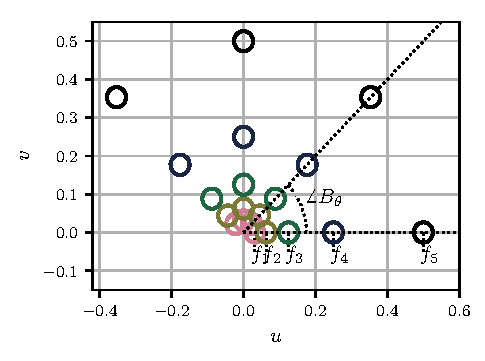
\includegraphics[width=0.49\textwidth]{GaborFilterbank_freq_2d_octave_spacing.pdf}}
    \subcaptionbox{\label{fig:2d_filterbank_half_crossingpoint}}{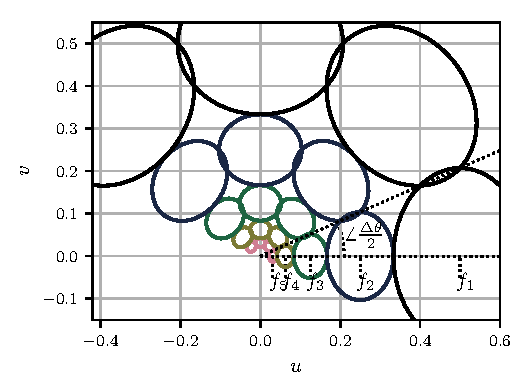
\includegraphics[width=0.49\textwidth]{GaborFilterbank_freq_2d_half_crossingpoint.pdf}}    
\caption{Filter spacing and crossing point effect represented on a 2-d filter bank in the frequency domain: \captext{(a)} Filters separation without crossing points between adjacent filters $[B_F=1, B_{\theta} = 45^{\circ}, \alpha=\beta=0.1, c_1=c_2=-]$, \captext{(b)} Filters separation with crossing points between adjacent filters $[B_F=1, B_{\theta} = 45^{\circ}, \alpha=f/\gamma, \beta=f/\eta, c_1=c_2=0.9]$. High and low cut-off frequency points given by $\Delta f$ and $\Delta \theta$ .}\label{fig:2d_filterbank_spacing}
\end{figure}

We know that for a filter whose center frequency is $f$ and whose cut-off angular interval is $\Delta \theta$, the full orientation bandwidth $B_\theta$ expressed in radians is defined as \citep{Daugman:JOSA:1985}.
\begin{equation}\label{eq:orientation_bandwidth_interval}
    B_{\theta} = 2 \tan^{-1} \left( \frac{\Delta \theta}{2f} \right)
\end{equation}

It is clear that using expression \eqref{eq:orientation_interval_crossing_point} in equation \eqref{eq:orientation_bandwidth_interval}, we find the expression that relates the frequency bandwidth to the central frequency and the length of the Gaussian minor axis.
\begin{equation}\label{eq:orientation_bandwidth}
    B_{\theta} = 2 \tan^{-1} \left( \frac{\beta}{\pi f} \sqrt{\ln \left(\frac{1}{c_2}\right)} \right)
\end{equation}

Taking the above relationships permits to write the 2-d GEF to use it into a bank as follows. 

\begin{equation}\label{eq:gabor_function_2d_spacefreq_bank}
    \begin{gathered}
         g(x,y) =  \frac{f^2}{\gamma \eta \pi} e ^{-\left(\frac{f^2}{\gamma^2} x_r^2 + \frac{f^2}{\eta^2} y_r^2\right)} e ^{j 2 \pi f x_r } \\
         G(u,v) =  e ^{-\left(\frac{\pi}{f}\right)^2\left( \gamma^2 (u_r-f)^2 + \eta^2 v_r^2\right)}
     \end{gathered}
\end{equation}
where now the length $\alpha$ of each filter in the bank will be determined based on the ratio $\gamma = \frac{f}{\alpha}$ and crossing point between adjacent filters $c_1$; and the length $\beta$ will be determined based on the ratio $\eta = \frac{f}{\beta}$ and crossing point between adjacent filters $c_2$.

Figure \ref{fig:2d_filterbank_spacing} shows the octave spacing and the orientation bandwidth for a bank of filters in the frequency domain. Particulary, figure \ref{fig:2d_filterbank_octave_spacing} shows a bank without the relationship between the effective width and the central frequency of the filter, whereas figure \ref{fig:2d_filterbank_half_crossingpoint} show the interdependence between $\alpha$, $\beta$, $B_F$, $B_{\theta}$, $f$ and the crossing points $c_1$, $c_2$.

\begin{figure}[!ht]
	\centering
	\begin{subfigure}[b]{0.8\textwidth}
		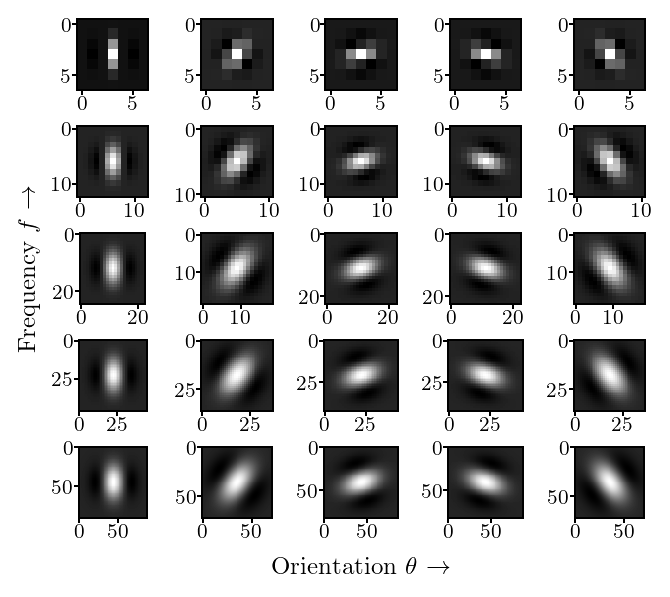
\includegraphics[width=\textwidth]{GaborFilterbank_spatial_2d_real}
		\caption{Real part}
		\label{fig:2d_filterbank_real}
	\end{subfigure}\\
	\begin{subfigure}[b]{0.8\textwidth}
		\centering
		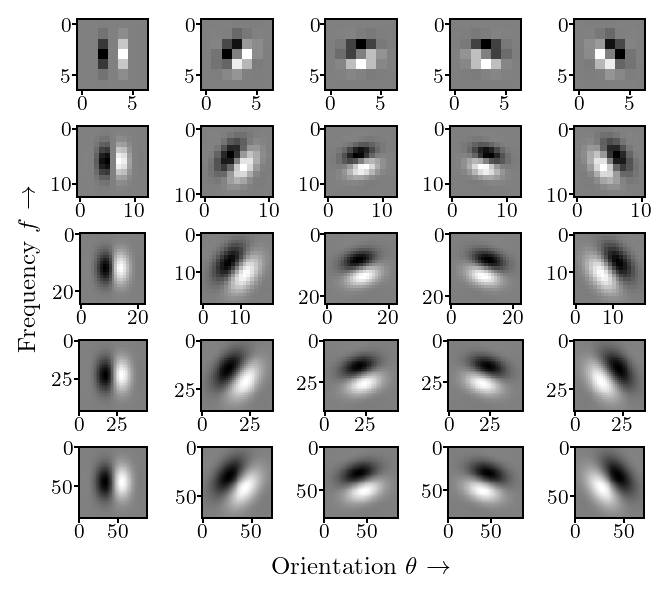
\includegraphics[width=\textwidth]{GaborFilterbank_spatial_2d_imag}
		\caption{Imaginary part}
		\label{fig:2d_filterbank_imag}
	\end{subfigure}
	    
    \caption{Custom designed Gabor filter bank. The design parameters are: max/min period $[1/f_{min}=70, 1/f_{max}=4]$, crossing points (frequency and angular) $[c_1=c_2= 0.9]$, bandwidths (frequency and angular) $[B_F=1, B_{\theta} = 35^{\circ}]$, standard devaitions $[\sigma=3]$.}\label{fig:2d_filterbank}
\end{figure}

\section{Conclusion}

In this chapter, we have presented a space-frequency analysis for creating a filter. This study aims to create a family of filters capable of measuring the texture information in an image under a perceptual approach. The human eye (perception and stimulus) is sensitive to the local contrast of textures, that is, to their amplitude. Therefore, we are interested in measuring this amplitude and its location correctly through a filter bank.

We use the Gabor function, which follows the Heisenberg uncertainty principle, to design an optimal filter bank. Given its ability to measure the texture's energy, both in the spatial and frequency domains, the filter configuration that we propose in this chapter allows us to build an adaptive filter bank. The filter bank is adaptable because we can customize it to privilege the precision of measuring the amplitude or the locality of a texture. Also, the proposed filter family is efficient since the Gaussian support is variable as a function of the central frequency of analysis, accelerating the convolution with the image.

On the other hand, each Gabor function of the filter bank is normalized concerning the central frequency of analysis, taking into account the size of the analysis window (Gaussian function). This characteristic makes it possible to attenuate the ripple and aliasing effects characteristic of the classic Gabor function.

The bank of filters proposed in this chapter achieves an almost total and uniform coverage of the frequency spectrum due to the modification of the frequency and angular crossover points.
We must then uniformly cover the entire spectrum. Modifying the Gabor function to create a filter bank is an effort to conceive filters capable of measuring the amplitude and locality of a texture's different spectral components. 

In the following chapters, we show this filter bank's use for the spectral decomposition of an image. This decomposition allows measuring the texture's information favoring the locality of the textures (without losing the amplitude), which makes this bank of filters a texture measurement tool.
